% Robin Prillwitz 2021
\documentclass[11pt,leqno,letterpaper]{article}

% Robin Prillwitz 2020

\usepackage[utf8]{inputenc}
\usepackage[T1]{fontenc}
\usepackage[ngerman]{babel}
\usepackage[autostyle,babel]{csquotes}

\usepackage{fontspec}
\newfontfamily\Verdana{Verdana}[Scale=MatchLowercase,
                                Ligatures=TeX]
\usepackage[iso,german]{isodate}
\usepackage{hyphenat}
\hyphenation{Mathe-matik wieder-gewinnen}

% japansese
% \usepackage{zxjatype}
% \setCJKmainfont{Hiragino Mincho ProN}


\usepackage{lipsum}

\usepackage{seqsplit}
\usepackage{tabto}
\usepackage{float}

\usepackage[margin=15pt,font=small,labelfont={bf,sf}]{caption}
\usepackage{subcaption}
\usepackage{wrapfig}
\usepackage{graphicx}
\usepackage{setspace}
\usepackage{multicol}
% \usepackage{kpfonts}
\usepackage[inline]{enumitem}
\usepackage{textcomp}
\usepackage{fullpage}
\usepackage{url}
\usepackage[usenames,dvipsnames,svgnames,table]{xcolor}
\usepackage{sectsty}
\usepackage{pdfpages}

\usepackage{bigfoot}
\interfootnotelinepenalty=10000

% TABLE
\usepackage{tabularx}
\newcolumntype{Y}{>{\centering\arraybackslash}X}

\definecolor{highlight}{rgb}{0.1882, 0.678, 0.8901}
\newcommand\hlc{\color{black}}
\chapterfont{\hlc}  % sets colour of chapters
\sectionfont{\hlc}  % sets colour of sections

\usepackage{tocloft}
\renewcommand{\cftsecleader}{\cftdotfill{\cftdotsep}}
\addto\captionsngerman{\renewcommand*\contentsname{\hlc Inhaltsverzeichnis}}

\usepackage[nottoc]{tocbibind}
\usepackage{fancyhdr}
\pagestyle{fancy}
\fancyhf{}
\renewcommand{\headrulewidth}{0pt}
\rfoot{\thepage}

% -- font styles
\usepackage{tgtermes}
% \usepackage[lf]{venturis}
% \usepackage{times}
\usepackage[sc]{mathpazo} % Palatino (very readable)
% \usepackage[adobe-utopia]{mathdesign}
% \usepackage{gfsdidot}
% \usepackage[scaled]{beraserif}
% \usepackage[bitstream-charter]{mathdesign}
% \usepackage{mathptmx}

% special math formatting
\usepackage{amsmath}
\usepackage{siunitx}

\floatstyle{ruled}

% -- structural elements
\newfloat{program}{thp}{lop}
\floatname{program}{Program}

% \newfloat{figure}{thp}{lop}
\floatname{figure}{Abbildung}

\renewcommand{\thetable}{\arabic{table}}
\renewcommand{\thefigure}{\arabic{figure}}

% -- syntax highlighting
\usepackage[scaled]{beramono}
\usepackage[T1]{fontenc}
\usepackage{color}
\usepackage{tabu}

\usepackage{tikz}
\usepackage{tikzpagenodes}
% \usepackage{pgfplots}
\usepackage{pgfplotstable}
\pgfplotsset{
  table/search path={./data},
}

\pagestyle{empty}
\usetikzlibrary{patterns}

\usepackage[
  left=2.5cm,
  right=2.5cm,
  top=3cm,
  bottom=2.5cm,
  includeheadfoot
]{geometry}

%% images
\usepackage{graphicx}
\usepackage{grffile}

\usepackage[toc,page]{appendix}
\renewcommand{\appendixpagename}{Anhang}
\renewcommand{\appendixtocname}{Anhang}


\usepackage{listings}
\usepackage{color}
\renewcommand\lstlistingname{Quelltext} % Change language of section name
\lstset{ % General setup for the package
    basicstyle=\small\sffamily,
    numbers=left,
    numberstyle=\tiny,
    frame=tb,
    tabsize=4,
    columns=fixed,
    showstringspaces=true,
    showtabs=false,
    showspaces=false,
    keepspaces,
    breaklines=true,
    commentstyle=\color{red},
    keywordstyle=\color{blue}
}

\usepackage[hidelinks]{hyperref}
% \urlstyle{same}
\urlstyle{tt}

% Robin Prillwitz 2020

% ----------------------------- biblatex w/ biber ---------------------------- %
\usepackage[
	backend=biber,
	natbib=true,
	% backref=true,
	% autocite=footnote,
	sorting=nyt,
	style=authoryear,
	% style=numeric,
	sortlocale=de_DE
]{biblatex}

% forbid pagebreaks in bib entry
\patchcmd{\bibsetup}{\interlinepenalty=5000}{\interlinepenalty=10000}{}{}

% ------------------------------- bib resouces ------------------------------- %
% \addbibresource[]{./references/test.bib}
\addbibresource{./references/references.bib}

% ------------------------------- localization ------------------------------- %
\DefineBibliographyStrings{ngerman}{%
		bibliography    = {Literaturverzeichnis},
		nodate          = {o.J.},
		backrefpage		 = {siehe Seite},% originally "cited on page"
		backrefpages	= {siehe Seiten},% originally "cited on pages"
		andothers		= {et al.}
}



% formatting & driver like
% https://www.scribbr.de/category/deutsche-zitierweise/
% -------------------------------- formatting -------------------------------- %
% \DeclareFieldFormat{editor}{#1}
% \DeclareFieldFormat{publisher}{#1}
% \DeclareFieldFormat{url}{[online]\ \url{#1}}
% \DeclareFieldFormat{urldate}{[#1]}


% ---------------------------------- drivers --------------------------------- %

% \DeclareBibliographyDriver{online}{%
%     \newunit%
%     \printnames{author}%
%     \ifnameundef{editor}%
%     {}%
%     {%
%         \newunit%
%         \printnames{editor}%
%     }%
%     \newunit\newblock%
%     :\ \printfield{title},%
%     \newunit\newblock%
%     \iffieldundef{publisher}%
%     {}%
%     {%
%         \ in \printfield{publisher},%
%         \newunit\newblock%
%     }%
%     \ \iffieldundef{year}%
%     {(o.J.)}%
%     {%
%         \printfield{year}%
%     },%
%     \newunit\newblock%
%     \newunit%
%     \printfield{url}%
%     \ \printurldate%
%     \newunit%
%     \finentry
% }

% \DeclareBibliographyDriver{book}{%
%     \newunit%
%     \printnames{author}:\ %
%     \newunit%
%     \printfield{title},%
%     \newunit\newblock%
%     \iffieldundef{editor}%
%     {}{%
%         \printnames{editor},%
%         \newunit\newblock%
%     }%
%     \iffieldundef{volume}%
%     {}{%
%         \printfield{volume},%
%         \newunit\newblock%
%     }%
%     \iffieldundef{edition}%
%     {}{%
%         \printfield{edition},%
%         \newunit\newblock%
%     }%
%     \iflistundef{location}%
%     {}{%
%         \printlist{location}:%
%         \newunit\newblock%
%     }%
%     \iflistundef{publisher}%
%     {}{%
%         \printlist{publisher},%
%         \newunit\newblock%
%     }%
%     % band auflage verlag jahr
%     \iffieldundef{year}%
%     {(o.J.)}%
%     {%
%         \printfield{year}%
%     }%
%     \newunit%
%     \finentry
% }

% Robin Prillwitz 2020

\usepackage[acronym, toc]{glossaries}
\usepackage[automake, nonumberlist, nogroupskip]{glossaries-extra}
\makeglossaries
\setabbreviationstyle[acronym]{long-short}

\newacronym{pwm}{PWM}{Pulse width modulation}
\newacronym{i2c}{I\textsuperscript{2}C}{Inter-IC Communication}
\newacronym{spi}{SPI}{Serial peripheral Interface}
\newacronym{ioctl}{IOCTL}{IO-Control}
\newacronym{ipc}{IPC}{Interprocess Communication}

\newacronym{cpu}{CPU}{Central Processing Unit (Prozessor)}
\newacronym{sbc}{SBC}{Single-Board Computer}
\newacronym{cli}{CLI}{Command Line Interface}

\newglossaryentry{rpi}{name={Raspberry Pi}, description={Ein kleiner \gls{sbc} für embedded Anwendungen}}
\newglossaryentry{float}{name={floating point}, description={32 oder 64-bit Gleitkommazahlen}}
\newglossaryentry{int}{name={integer}, description={32 oder 64-bit Ganze, natürliche, Zahlen}}

% cursive acronyms
\renewcommand*{\glstextformat}[1]{\textit{#1}}
% glossary spaceing
\renewcommand\glstreepredesc{\tabto{4cm}}

\makeglossaries


\def \faculty   {Angewandte Informatik}
\def \degree    {Angewandte Informatik}
\def \title     {Lüftersteuerung mit Temperatursensor}
\def \type      {Projektarbeit}
\def \class     {AI-B6-Systemprogrammierung}
\def \semester  {SS2022}

\def \auditor   {Prof. Bösnecker}

\def \authorA    {Robin Prillwitz}
\def \matrnrA    {00805291}

\def \zipA       {84326}
\def \locationA  {Falkenberg}

\def \authorB    {Sven Menzel}
\def \matrnrB    {00804260}

\def \zipB       {93073}
\def \locationB  {Neutraubling}

\def \date      {\today}

\def \stretch {1}

\begin{document}
\setstretch{1.0}

% HEADING
% Robin Prillwitz 2020

\newgeometry{
    left=1.50cm,
    right=1.50cm,
    top=1.11cm,
    bottom=2cm
}
\begin{titlepage}
    \thispagestyle{empty}
    % draw outline
    \begin{tikz}[remember picture,overlay]
        \draw[black, line width=1pt]
        (current page text area.south west) rectangle
        (current page text area.north east);
    \end{tikz}
    % write text stuff
    \begin{center}
        {
        \Verdana
        \fontsize{14}{14.4}\selectfont
        \vspace{2.4cm}
        Technische Hochschule Deggendorf\\
        \vspace{2cm}
        Fakultät \faculty\\
        (Bachelor-Studiengang \degree)\\
        \vspace{3cm}
        \textbf{\title}\\
        \vspace{3.8cm}
        \type \\ für das\\ \class\\ \semester\\
        \vspace{3.8cm}
        \fontsize{14}{24.4}\selectfont
        % lower two column stuff
        \begin{tabularx}{0.9\textwidth}{
            >{\hsize=0.9\hsize\linewidth=\hsize}X
            >{\hsize=0.5\hsize\linewidth=\hsize}X
        }
            vorgelegt von: & Erstprüfer: \\
            \authorA\;(\matrnrA), \zipA\;\locationA & \underline{\hspace*{5.5cm}} \\
            \authorB\;(\matrnrB), \zipB\;\locationB & \\
            am: \date &
        \end{tabularx}
        }
    \end{center}
\end{titlepage}
\restoregeometry
\newpage


\setcounter{page}{1}
\pagenumbering{roman}
% TOC
% \addcontentsline{toc}{section}{Inhaltsverzeichnis}%
% \thispagestyle{empty}
\tableofcontents
\thispagestyle{fancy}
% TABLES
\newpage
\listoftables
\thispagestyle{fancy}
% \thispagestyle{empty}
% FIGURES
\listoffigures
\thispagestyle{fancy}
% \thispagestyle{empty}
\thispagestyle{fancy}
% \newpage
% ACRONYMS
\setglossarystyle{listdotted}
\setglossarystyle{tree}
% \printacronyms[]
\printglossary[type=\acronymtype, title=Abkürzungsverzeichnis]
\printglossary
% \thispagestyle{empty}
\thispagestyle{fancy}

\newpage
\setcounter{page}{1}
\pagenumbering{arabic}
\pagestyle{fancy}

\setstretch{\stretch}

% ----------------------

\section{Motivation}
% Im sechsten Semesters des Studiengangs Angewandte Informatik wird im Fach Systemprogrammierung die Anwendung eines Linux Treibers gelehrt.
% Hierbei entsteht die Möglichkeit die Kenntnisse der Treiberprogrammierung im Rahmen einer Prüfungsstudienarbeit weiter zu vertiefen.

Das Thema dieser Studienarbeit ist die Programmierung eines Gerätetreibers für Linux.
Dieses Projekt implementiert eine Lüftersteuerung mit Temperatursensor.
Zum Einsatz kommen ein \gls{rpi} 4b, ein Noctua \textit{NF-A4x20} 5V \gls{pwm} Lüfter mit vier Pins und ein digitaler Temperatursensor \texttt{TMP102}.
Der Temperatursensor misst die momentane Umbgebungstemperatur.
Je nach Erwärmung wird die Drehgeschwindigkeit des Lüfters beeinflusst.
Hierbei versucht der Lüfter die Temperatur um den Temperatursensor auf normale Umgebungstemperatur herunter zu kühlen.

Das Projekt besteht aus der Applikation im Userspace und dem Treiber im Kernelspace.
Der Treiber kommuniziert mit \gls{i2c} und \gls{spi} mit Hardwarepäripherie.
Die Schnittstelle zwischen Kernelspace und Userspace wird durch sowohl \gls{fops} und \gls{ioctl} ermöglicht.
\autoref{fig:block} beschreibt den abstrakten Aufbau des Projekt.
Im Folgenden Dokument wird der Aufbau von sowohl der Software als auch der Hardware erklärt.

\begin{figure}[h]
    \centering
    \begin{tikzpicture}
        \draw (0,1) node {};
        \draw (0,-10) node {};
        \draw[fill=black!20!white, draw, thick] (-3,0.5) rectangle ++(6cm,-5cm);
        \node[fill=red!40!white, thick, draw, minimum height=1cm, minimum width=6cm] (app) {Applikation (Userspace)};
        \node[minimum height=1cm, minimum width=6cm, below of=app] (fops) {\acrshort{fops} oder \acrshort{ioctl}};
        \node[fill=red!40!white, thick, draw, minimum height=1cm, minimum width=5cm, below of=fops] (driver) {Fanctrl (Kernelspace)};
        \node[minimum height=1cm, minimum width=6cm, below of=driver] (kernel) {Linux Kernel};
        \node[fill=black!20!white, thick, draw, minimum height=1cm, minimum width=6cm, below of=kernel] (hardware) {\gls{rpi} Hardware};
        \node[below= 1cm of hardware] (sensor) {};
        \node[fill=red!40!white, thick, draw, minimum height=1cm, minimum width=3cm, left = 0.2cm of sensor] (tmp) {\texttt{TMP201}};
        \node[fill=red!40!white, thick, draw, minimum height=1cm, minimum width=3cm, right = 0.2cm of sensor] (mcp) {\texttt{MCP41XXX}};
        \node[fill=red!40!white, thick, draw, minimum height=1cm, minimum width=3cm, below of=mcp] (pwm) {\texttt{555} PWM};
        \node[fill=black!20!white, thick, draw, minimum height=1cm, minimum width=6cm, below = 2cm of sensor] (fan) {Lüfter};
        \draw[black, very thick, ->] (pwm) -- ++(0,-1.15cm) node[above left] {\acrshort{pwm}};
        \draw[black, very thick, <-] (tmp) -- ++(0,-2.15cm) node[left, pos=0.5] {Luft};

        \draw[black, very thick, <-] (mcp) -- ++(0,1.15cm) node[below left] {\acrshort{spi}};
        \draw[black, very thick ,<->] (tmp) -- ++(0,1.15cm) node[below left] {\acrshort{i2c}};
        \draw[black, thick, ->] (-4cm, 0) node[left] {Hohe Abstraktion} -- ++(0,-3cm) node[left] {Niedrige Abstraktion};
        \draw[black, thick] (-4cm, -4cm) -- ++(0,-5cm) node[left, pos=0.5] {Hardware};
    \end{tikzpicture}
    \caption[Blockschaltbild des \texttt{Fanctrl} Projekts]{Blockschaltbild des \texttt{Fanctrl} Projekts. Die in rot abgebildeten Lagen sind eigens implementiert.}
    \label{fig:block}
\end{figure}

\clearpage
\section{Hardware}

\subsection{Temperatursensor}
\subsubsection{Hardwareanschluss}
\subsubsection{I\textsuperscript{2}C Bus}

\subsection{\Acrshort{pwm}-Erzeugung}

Um die Geschwindigkeit eines Lüfters zu regulieren, wird dieser mit einem \gls{pwm} Signal gesteuert.
Die Pulsweite ist proportional zur resultierenden Zielgeschwindigkeit.
Der \gls{rpi} hat interne Hardware um \gls{pwm} Signale zu generieren.
Diese sind jedoch nicht trivial aus dem Kernelspace erreichbar.

Als Ersatzlösung wird externe Hardware genutzt.
Ein \texttt{555} Timer erstellt ein rechteckiges Wechselsignal.
Die Pulsweite wird durch ein \texttt{MCP41XXX} digitales Potentiometer über \gls{spi} eingestellt.
Folglich ist die Lüftergeschwindigkeit proportional zur Pulsweite und proportional zum eingestellten Wiederstand.

\subsubsection{SPI Bus}

SPI ist ein synchroner, serieller Datenbus mit der Funktionsweise nach dem Master-Slave-Prinzip.
Die vier wichtigsten Leitungen sind \gls{sclk}, \gls{mosi}, \gls{miso} und \gls{ss}.
Die \gls{sclk} gibt einen Takt mit einer möglichen Frequenz bis $\si{\mHz}$ aus, welche zur Synchronisation vom Controller benötigt wird. Dieses Signal wird vom Master ausgegeben.
Mit \gls{ss} wird der jeweilige Slave ausgewählt, indem das Signal auf logisch 0 gesetzt wird.
Daten werden mit der \gls{mosi} Leitung vom Master zum Slave und mit der \gls{miso} Leitung vom Slave zum Master gesendet. \\
In \autoref{fig:spi-transaction} ist die Funktion von \gls{spi} dargestellt.
Wenn der Slave ausgewählt wurde, toggelt der \gls{ss} von logisch 1 auf logisch 0.
Mit jedem \gls{sclk} Takt wird ein Bit von Master auf Slave übertragen.
Nach Beenden der Übertragung toggelt der \gls{ss} wieder auf logisch 1.
Dies funktioniert mit der \gls{miso} Leitung vice versa.

\begin{figure}
    \begin{center}
    \begin{tikztimingtable}[%
        timing/dslope=0.2,
        timing/.style={x=1.6ex,y=2ex},
        x=1ex,
        timing/rowdist=4ex,
        timing/c/rising arrows,
        timing/name/.style={font=\sffamily\scriptsize},
    ]
    \busref{CS} & HHL;16{L};LHH\\
    \busref{SCK} & UULL;16{C};UU\\
    \busref{SO} & UUU;2D{D7};2D{D6};2D{D5};2D{D4};2D{D3};2D{D2};2D{D1};2D{D0};UUU\\
    %
    \extracode
    \begin{pgfonlayer}{background}
        \begin{scope}[semitransparent ,semithick]
            \vertlines[darkgray,dotted]{0,3.2 ,...,36.0}%
        \end{scope}
        \end{pgfonlayer}
    \end{tikztimingtable}
    \end{center}
    \caption[Eine \gls{spi} Datenübertragung.]{Eine \gls{spi} Datenübertragung von 8 Bits}
    \label{fig:spi-transaction}
\end{figure}

\subsubsection{MCP41XXX Digitales Potentiometer}

Die Schaltung des digitalen Potentiometers wird direkt an den \gls{rpi} angeschlossen.
Die Pins werden wie in \autoref{tab:spi} verbunden.
Der \texttt{MCP41XXX} hat zwei interne digital steuerbare Potentiometer.
Um deren Wiederstandswert einzustellen müssen zwei Bytes über \gls{spi} gesendet werden.
Das erste Byte stellt das Command-Byte dar.
Das zweite Byte die tatsächlichen Daten.
Die in \autoref{fig:spi-mcp-transaction} aufgeführten Bits in der Datenübertragung setzen sich aus dem Command-Byte und aus einem folgenden Datenbyte zusammen.
Die Bedeutung des Command-Byte wird in \autoref{tab:command-bits} erklärt.
Das Datenbyte setzt sich aus den folgenden 8 Bits (D7, \ldots, D0) zusammen.
Der resultierende Wiederstand zwischen Anschluss A und W kann mit der \autoref{eq:resistance1} berechnet werden.
Der Wiederstand zwischen B und W ist mit \autoref{eq:resistance2} zu berechnen.

\begin{table}[h]
    \centering
    \begin{tabular}{|r||l|l|l|l|l|}
        \hline
        \textbf{Funktion} & \textbf{\acrshort{mosi}} & \textbf{\acrshort{miso}} & \textbf{\acrshort{vcc}} & \textbf{\acrshort{sclk}} & \textbf{\acrshort{ss}} \\
        \hline
        \hline
        \gls{rpi} Pin Name & GPIO10 & GPIO9 & 5V Power & GPIO11 & GPIO8 \\
        \hline
        \gls{rpi} Pin Nummer & Pin19 & Pin21 & Pin2 & Pin23 & Pin24 \\
        \hline
    \end{tabular}
    \caption{\gls{spi} Pinout Tabelle}
    \label{tab:spi}
\end{table}

\begin{figure}[h]
    \begin{center}
    \begin{tikztimingtable}[%
        timing/dslope=0.2,
        timing/.style={x=1.6ex,y=2ex},
        x=1ex,
        timing/rowdist=4ex,
        timing/c/rising arrows,
        timing/name/.style={font=\sffamily\scriptsize},
    ]
    \busref{CS} & HHL;32{L};LHH\\
    \busref{SCK} & UULL;32{C};UU\\
    \busref{SO} & UUU;2D{X};2D{X};2D{C1};2D{C0};2D{X};2D{X};2D{P1};2D{P0};2D{D7};2D{D6};2D{D5};2D{D4};2D{D3};2D{D2};2D{D1};2D{D0};UUU\\
    %
    \extracode
    \begin{pgfonlayer}{background}
        \begin{scope}[semitransparent ,semithick]
            \vertlines[darkgray,dotted]{0,3.2 ,...,36.0}%
        \end{scope}
        \end{pgfonlayer}
    \end{tikztimingtable}
    \end{center}
    \caption[Eine \gls{spi} Datenübertragung für ein MCP41XXX Potentiometer]{Eine \gls{spi} Datenübertragung für ein MCP41XXX Potentiometer}
    \label{fig:spi-mcp-transaction}
\end{figure}

\begin{table}[h]
    \centering
    \begin{subtable}[t]{5cm}
        \centering
        \begin{tabular}{|l|l|l|}
            \hline
            \textbf{C1} & \textbf{C0} & \textbf{Kommando} \\
            \hline
            \hline
            0 & 0 & Kein Kommando \\
            \hline
            0 & 1 & Daten Schreiben \\
            \hline
            1 & 0 & Ausschalten \\
            \hline
            1 & 1 & Kein Kommando \\
            \hline
        \end{tabular}
        \caption{Kommando Bits}\label{command:1a}
    \end{subtable}
    \quad
    \begin{subtable}[t]{5cm}
        \centering
        \begin{tabular}{|l|l|l|}
            \hline
            \textbf{P1} & \textbf{P0} & \textbf{Kommando} \\
            \hline
            \hline
            0 & 0 & Kein Potentiometer \\
            \hline
            0 & 1 & Nur Potentiometer 0 \\
            \hline
            1 & 0 & Nur Potentiometer 1 \\
            \hline
            1 & 1 & Beide Potentiometer \\
            \hline
        \end{tabular}
        \caption{Potentiometer bits}\label{command:1b}
    \end{subtable}
    \caption{MCP41XXX Command-Byte Bits}
    \label{tab:command-bits}
\end{table}

\begin{samepage}
\begin{equation}
    R_{\text{\text{WA}}}(D_{\text{n}}) = \frac{(R_{\text{AB}}) (256 - D_{\text{n}})}{256} + R_{\text{W}}
    \label{eq:resistance1}
\end{equation}
\begin{equation}
    R_{\text{WB}}(D_{\text{n}}) = \frac{(R_{\text{AB}}) (D_{\text{n}})}{256} + R_{\text{W}}
    \label{eq:resistance2}
\end{equation}
wobei
\begin{align*}
    R_{\text{AB}} &: \text{Wiederstand zwischen Anschluss A und B, hier: } 10\si{k\ohm} \\
    R_{\text{W}} &: \text{Wiper Wiederstand, nominal: } 52\si{\ohm}  \\
    D_{\text{n}} &: \text{Dezimalwert des Wiperregisters: } 0_{10} \leq D_{\text{n}} \leq 255_{10}
\end{align*}
\end{samepage}

\subsubsection{555 Timer}

Der Timer ist in einer astabilen Konfiguration verbunden.
Der Timer erwartet lediglich eine positive Spannung über $U+$ zu $U-$ von $3.3\si{\volt}$.
Ein rechteckiges Ausgangssignal mit einstellbarer Pulsweite wird an Pin 7, \texttt{DIS}, oder auch an Pin 3, \texttt{OUT}, gegben.
\texttt{DIS} ist Open-Drain womit der High-Pegel zu einer beliebigen Spannung eingestellt werden kann.
Eine analytische Bestimmung von $U_C(t)$ oder $I(t)$ kann aufgrund der nicht linearen Übertragungsfunktion der Diode nicht bestimmt werden \autocite{rdc}.
Folglich ist eine Berechnung von $f$ nicht möglich\footnote{Eine grobe Annäherung durch die Annahme, dass $U_{fd}$ der Dioden konstant und unabhängig von $I$ ist, ist möglich, jedoch sind die resultate daraus sehr ungenau und nahezu unbrauchbar.}.
Die Frequenz kann lediglich empirisch durch Messung oder Simulation ermittelt werden.
Der \texttt{LTSpice} Quellcode für die Partielle Bestimmung der Spannung an dem Kondensator wird in \autoref{apx:sim} gegeben.
Der Duty-Cycle des \gls{pwm} Signals kann nicht analytisch bestimmt werden, jedoch ist dieser proportional zu den Wiederständen ($R_{\text{WA}} \propto D, R - R_{\text{WB}} \propto D$).
Diese Annahme wird auch in dem Treiber genutzt.

\begin{figure}[p]
    \centering
    \begin{tikzpicture}[
        %Global Config
        font=\small
    ]
    %You can create an smart objet like Henry Menke in this post http://www.texample.net/tikz/examples/4-bit-counter/
    % Variables: 1: Position 2: ID.
    \def\TIMER555(#1)#2{%
    \begin{scope}[shift={(#1)}]
        \draw[fill=blue!10] (-1.5,-2) rectangle (1.5,2); % The body of IC
        % Label and component identifier.
        % \draw[blue] (2,2.5) node []{\large \bf U - #2}; % IC LABEL
        \draw[blue] (0,0.5) node [align=center]{\large NE-555\\TIMER}; % IC LABEL
        % Draw the pins
        % Some that you have to learn about label nodes, draw lines, and name coordinates in Tikz
        \draw (0.9,-2) node [above]{GND} -- +(0,-0.5) node [anchor=-45]{1} coordinate (#2 GND); % Pin 1 GND
        \draw (-1.5,-1.5) node [right]{TRG} -- +(-0.5,0) node [anchor=-135]{2} coordinate (#2 TRG); % Pin 2 TRG
        \draw (1.5,0) node [left]{OUT} -- +(0.5,0) node [anchor=-45]{3} coordinate (#2 OUT); % Pin 3 OUT
        \draw (0.9,2) node [below]{RESET} -- +(0,0.5) node [anchor=45]{4} coordinate (#2 RESET); % Pin 4 RESET
        \draw (0,-2) node [above]{CTRL} -- +(0,-0.5) node [anchor=-45]{5} coordinate (#2 CTRL); % Pin 5 CTRL
        \draw (-1.5,-.5) node [right]{THR} -- +(-0.5,0) node [anchor=-135]{6} coordinate (#2 THR); % Pin 6 THR
        \draw (-1.5,1.5) node [right]{DIS} -- +(-0.5,0) node [anchor=-135]{7} coordinate (#2 DIS); % Pin 7 DIS
        \draw (0,2) node [below]{$\mathsf{V_{CC}}$} -- +(0,0.5) node [anchor=45]{8} coordinate (#2 VCC); % Pin 8 VCC
    \end{scope}
    }

    \TIMER555(0,0){1}

    \draw (-9,4) node[ocirc] (VCC){} node[left]{${U+}$};
    \draw (-9,-4) node[ocirc] (GND){} node[left]{${U-}$};

    \draw(VCC)to [short, o-] ++(1,0) coordinate (NOD1);

    \draw (-8, 2) to[potentiometer, n=mcp, l_=$R$] ++(2,0);
    \draw (mcp.a) node[above right] {$B$};
    \draw (mcp.b) node[above left] {$A$};
    \draw (mcp.wiper) node[right] {$W$};
    \draw (1 OUT) -- ++(1,0)-- ++(0, 5) -| (mcp.wiper);
    \draw (mcp.b)--++(-1, 0) to[D,n=d1,l_=$D_1$] ++(0,-2);
    \draw (mcp.a)--++(1, 0) to[D,invert, n=d2,l_=$D_2$] ++(0,-2) -| (d1.a);
    \draw (mcp) to[open, -*] ++(0,-2) -- ++(0,-2) coordinate (NOD2) to[C,n=C,l_=$C$, -*] (mcp |- GND);

    \draw(1 TRG) --++(-1,0);
    \draw(1 THR) --++(-1,0) to[short, -*] ++(0,-1) to[short, -*] ++(-4,0);

    \draw(1 VCC) to [short, -*] (1 VCC |- NOD1);
    \draw(1 RESET) to [short] (1 RESET |- NOD1) to [short] (NOD1);

    \draw(1 CTRL) to [C,l_=100nF, -*] (1 CTRL |- GND);
    \draw(1 GND) to [short] (1 GND |- GND) to [short] (GND);

    \draw(1 DIS)--++(-1,0) to[R, *-*, l_={$5,6\si{k\ohm}$}] ++(0,2.5);
    \draw(1 DIS)++(-1,0) to[short] ++(-1,0) node[ocirc](OUT){} node[below]{PWM};

    \end{tikzpicture}
    \caption{NE555 Timer in PWM Konfiguartion.}
    \label{fig:ne555-pwm}
\end{figure}

\subsubsection{Lüfterkontrolle mit \acrshort{pwm}}

Zur Kühlung wird ein \textit{NF-A4x20} 4-Poliger \gls{pwm} Lüfter von \textit{Noctua} aus \autoref{fig:fan-pic} verwendet.
Dieser benötigt eine Gleichspannung von $5\si{\volt}$ und wird mit einem \gls{pwm} Signal mit einer Amplitude von $5\si{\volt}$ angesteuert.
Das Tacho-Signal wird nicht verwendet.
Die Pins werden wie in \autoref{tab:fan-pinout} verbunden.

\begin{figure}[p]
    \centering
    \begin{subfigure}{0.4\textwidth}
        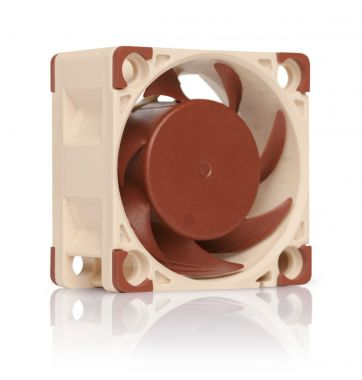
\includegraphics[width=6cm]{./pic/noctua-1.jpg}
    \end{subfigure}
    \begin{subfigure}{0.4\textwidth}
        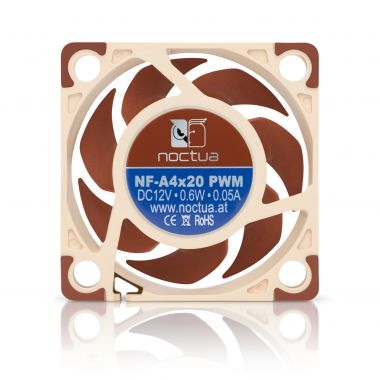
\includegraphics[width=6cm]{./pic/noctua-2.jpg}
    \end{subfigure}
    \caption{Der Lüfter von \textit{Noctua} \autocite{noctua-fan}.}
    \label{fig:fan-pic}
\end{figure}

\begin{table}[p]
    \centering
    \begin{tabular}{|l|l|l|l|}
        \hline
        \textbf{Lüfter Pin} & \textbf{Farbe} & \textbf{Funktion}  & \textbf{Anschluss} \\
        \hline
        \hline
        1 & \textcolor{black}{$\blacksquare$ Schwarz} & \gls{gnd} & \gls{gnd} \\
        \hline
        2 & \textcolor{Goldenrod}{$\blacksquare$ Gelb} & \gls{vcc} & $5\si{\volt}$ \\
        \hline
        3 & \textcolor{ForestGreen}{$\blacksquare$ Grün} & Tach & \gls{nc} \\
        \hline
        4 & \textcolor{blue}{$\blacksquare$ Blau} & \gls{pwm} & \gls{pwm} von \texttt{555} \\
        \hline
    \end{tabular}
    \caption{\gls{pwm} Lüfter Pinout Tabelle}
    \label{tab:fan-pinout}
\end{table}


\clearpage
\section{Software}

\subsection{Kernel Treiber}

\begin{wrapfigure}[25]{o}[1cm]{8cm}
\dirtree{%
.1 /.
.2 install\_driver.sh.
.2 .gitignore.
.2 README.md.
.2 doc/.
.2 app/.
.2 driver/.
.3 Makefile.
.3 spidev\_disabler.dts.
.3 src/.
.4 fanctrl.c.
.4 fanctrl.h.
.4 fops.c.
.4 fops.h.
.4 pwm.c.
.4 pwm.h.
.4 temp.c.
.4 temp.h.
.4 ioctl.c.
.4 ioctl.h.
}
\caption{Ordnerstruktur des Treibers}
\label{fig:driverdirectory}
\end{wrapfigure}

Der Code des Kernel-Treibers ist in \texttt{C99} geschrieben.
Dieser ist Prozessoragnostisch.
Es werden jedoch existierende low-level Treiber zwischen den Prozessorregistern und Kerenlspace erwartet, die die Kommunikation über \gls{i2c} und \gls{spi} abstrahieren.
Das Modul an sich ist lediglich von linux-Headern abhängig.
Der Treiber ist auf verschiedene \texttt{C}-Dateien aufgeteilt.
Die Struktur des Treibers ist in \autoref{fig:driverdirectory} aufgeführt.
Der Tatsächliche Quellcode für den Treiber befindet sich lediglich im \texttt{src} Ordner.
Alle anderen Dateien sind notwendig jedoch kein direkter Teil des Treibers.

Die Haupt-Datei mit dem Anfangspunkt des Treibers ist in \texttt{fanctrl.c}.
Darin wird das Treibermodul initialisiert, registriert, ausgeführt und schließlich auch de-initialisiert.
Der Kernel-Treiber kann über sowohl durch \gls{fops} als auch mit \gls{ioctl} mit dem Userspace kommunizieren.
Dies wird in den \texttt{fops.c} und \texttt{ioctl.c} und deren jehweils dazugehörigen Header-Files implementiert.
Die anderen zwei Hauptfunktionen, die Kommunikation über \gls{i2c} und \gls{spi} werden in \texttt{temp.c} und \texttt{pwm.c} respektiv implementiert.
In den folgenden Abschnitten werden die implementierten Funktionen, zusätzliche Dateien und der Kompilierungs/Installationsvorgang beschreiben.

\subsubsection{Temperatursensor über \acrshort{i2c}}

Der Temperatursensor ist in \texttt{./src/temp.c} und \texttt{./src/temp.h} implementiert.
Mit der Funktion \texttt{tempInit} wird der \gls{i2c} Adapter initialisiert.
Dannach wird ein neuer \gls{i2c} Device struct hinzugefügt und der Treiber wird dem Adapter registriert.
Der Device beinhält die Informationen über Device Name und Addresse.
Ist der Adapter initialisiert wird dieser mit \texttt{tempDeinit}zum Programm Ende, falls er erfolgreich initialisiert wurde, wieder deinitialisiert.
Dabei werden alle vom \gls{i2c} Adapter genutzen Ressourcen für den Treiber frei gegeben.
Auf dem \gls{rpi} muss \gls{i2c} durch die \texttt{raspi-config} aktiviert werden.

Der \texttt{TMP102} Sensor gibt Messdaten mit 13-Bit Präzision bei einer Auflösung von $0.0625\si{\degree C}$ am \gls{lsb} an.
Um einen Messwert zu einer Temperatur zu konvertieren müssen zuerst zwei Byte gelesen werden.
Diese müssen zu einem 16-Bit Wert, welcher den ogrinellen 13-Bit Messwert beinhaltet, konkatiniert werden.
Anschlie{\ss}end muss der Messwert linear abgebildet werden, dass hei{\ss}t mit der Auflösung pro \gls{lsb} multiplizieren.
Die \gls{fpu} sollte unter allen Umständen nicht aus dem Kernelspace verwendet werden,
da die Kontextänderung abträgliche Performanceimplikationen auf Userspace Applikationen mit sich führen kann.
Die berechnung wird folglich mit der Integerdivision des Kehrwerts wie in \autoref{eq:temp-convert} ausgeführt.
Der Fehler der Berechnung wird in \autoref{eq:temp-error} aufgeführt und in \autoref{fig:rounding-err} visualisiert.
Der resultierende Rundungsfehler manifestiert sich als Rauschen.
Da unsere Anwednung sich nominal bei und über Raumtemperatur in Einer-Stellen Präzision agiert sind die resultierenden Fehler vernachlässigbar.
Die Implementation der Kommunikation mit dem Sensor und Wandlung der Daten ist in \autoref{code:i2c-convert} gegeben.

\begin{equation}
    \vartheta = \texttt{M}_D \cdot 0.0625\si{\celsius} = \frac{\texttt{M}_D}{\left(0.0625\si{\celsius}\right)^{-1}} = \frac{\texttt{M}_D}{16\si{\per\celsius}} \approx \left\lfloor\frac{\texttt{M}_D}{16\si{\per\celsius}}\right\rfloor
    \label{eq:temp-convert}
\end{equation}
\begin{equation}
    \begin{aligned}
        \Delta_{\texttt{M}_D} &= \frac{\texttt{M}_D}{16\si{\celsius}} - \left\lfloor\frac{\texttt{M}_D}{16\si{\per\celsius}}\right\rfloor \\[2ex]
        \delta_{\texttt{M}_D} &= \frac{\Delta_{\texttt{M}_D}}{\frac{\texttt{M}_D}{16\si{\celsius}} }\\[2ex]
    \end{aligned}
    \label{eq:temp-error}
\end{equation}

\lstinputlisting[linerange=i2c\ read\ start-i2c\ read\ end, caption={\texttt{./driver/src/temp.c} \gls{i2c} Daten auslesen}, label=code:i2c-convert, float=h]{../../driver/src/temp.c}

\begin{figure}[h]
    \centering
    \begin{subfigure}[b][7cm][t]{10cm}
        \centering
        \begin{tikzpicture}
            \begin{axis}[%
                xmin=0,
                xmax=2400,
                ymin=-1.5,
                ymax=1.5,
                samples=3000,
                width=10cm,
                height=7cm,
                minor tick num=5,
                grid=both,
                grid style={line width=.1pt, draw=gray!10},
                major grid style={line width=.2pt,draw=gray!50},
                % nodes near coords,
                xlabel near ticks,
                xticklabel style={rotate=45,anchor=north east,inner sep=0mm},
                xlabel={$\texttt{M}_D$},
                ylabel={\textcolor{red}{$\Delta_{\texttt{M}_D}$}, \textcolor{blue}{$\delta_{\texttt{M}_D}$} von $\vartheta$},
                ylabel near ticks]
                % \addplot[domain=0:6.4, blue, very thick, smooth, ->] {2.1971*1.8206^x};
                \addplot[domain=0:2400, red] {(x * 0.0625) - round(x / 16)};
                \addplot[domain=0:2400, blue] {((x * 0.0625) - round(x / 16)) / (x * 0.0625)};
            \end{axis}
        \end{tikzpicture}
    \end{subfigure}
    \begin{subfigure}[b][7cm][t]{4cm}
        \centering
        \begin{tikzpicture}
            \begin{axis}[%
                xmin=0,
                xmax=100,
                ymin=-1.5,
                ymax=1.5,
                samples=500,
                width=5cm,
                height=7cm,
                minor tick num=5,
                grid=both,
                grid style={line width=.1pt, draw=gray!10},
                major grid style={line width=.2pt,draw=gray!50},
                % nodes near coords,
                xlabel near ticks,
                xticklabel style={rotate=45,anchor=north east,inner sep=0mm},
                xlabel={$\texttt{M}_D$},
                ymajorticks=false]
                % \addplot[domain=0:6.4, blue, very thick, smooth, ->] {2.1971*1.8206^x};
                \addplot[domain=0:100, red] {(x * 0.0625) - round(x / 16)};
                \addplot[domain=0:100, blue] {((x * 0.0625) - round(x / 16)) / (x * 0.0625)};
            \end{axis}
        \end{tikzpicture}
    \end{subfigure}
    \caption[Integerdivisionsinduzierter Rundungsfehler]{Integerdivisionsinduzierter Rundungsfehler der Temperatursensorkonversion aus \autoref{eq:temp-error}.
    \textcolor{red}{Rot: Absoluter Fehler $\Delta_{\texttt{M}_D}$.}
    \textcolor{blue}{Blau: Relativer Fehler $\delta_{\texttt{M}_D}$.}
    }
    \label{fig:rounding-err}
\end{figure}

\subsubsection{Potentiometer über \acrshort{spi}}
\subsubsubsection{\acrshort{spi} Implementation}

Die Initialisierung des \gls{spi} Treibers läuft sehr ähnlich zu der des \gls{i2c} Treibers ab.
Die genaue Implementation ist in \texttt{./src/pwm.c} und \texttt{./src/pwm.h} zu finden.
Es wird zuerst ein \texttt{spi\_board\_info} struct angelegt, welches mit den relevanten Daten des \gls{sbc} gefüllt wird.
Dazu zählen die Nummer des Kernel \gls{spi} Treibers, dessen \gls{ss} Signal Nummer und dessen Geschwindigkeit.
Diese ist hier als $4\si{\mega\hertz}$ festgelegt.
Dannach wird mit der Funktion \texttt{spi\_busnum\_to\_master} ein geeignerter Bus Master gesucht.
Diser Master implementiert die Schnittstelle zwischen dem Kernel und der Hardware.
Folgend wird mit \texttt{spi\_new\_device} und schließlich \texttt{spi\_setup} ein \gls{spi} Device angelegt und registriet.
Zu jedem Schritt können Fehler auftreten, welche abgefangen werden.
Die Deinitialisierung verläuft wieder ähnlich.
Ist der \gls{spi} Device erfolgreich geladen, so wird dieser einfach mit \texttt{spi\_unregister\_device} unregistriert.

Um den Wiederstand des Potentiometers zu setzen, wird die in \autoref{code:spi-write} gezeigte Funktion genutzt.
Darin wird eine \gls{spi} Transaktion aus zwei Bytes erstellt.
Der \texttt{MCP} Chip erwartet zuerst das \textit{Command Byte} in Form von \autoref{tab:command-bits}.
Im Code ist dieses als \texttt{0b00010011} festgelegt.
Dadurch werden beide internen Potentiometer das dannach folgende Byte in das interne Register laden.
Da der Duty Cycle propotional und relativ zu dem Wiederstand ist, kann hier der Wert für das Wiederstandsregister auch als Prozentbereich wie in \autoref{eq:interpret} interpretiert werden.
\begin{equation}
    \left[0_{\text{H}}; FF_{\text{H}}\right] \rightarrow \left[0\%; 100\%\right]
    \label{eq:interpret}
\end{equation}

\lstinputlisting[linerange=spi\ write\ start-spi\ write\ end, caption={\texttt{./driver/src/pwm.c} \gls{spi} Potentiometer setzen}, label=code:spi-write, float=h]{../../driver/src/pwm.c}

\subsubsubsection{Devicetree Overlay}
Auf dem \gls{rpi} muss der \gls{spi} Treiber durch \texttt{raspi-config} aktiviert werden.
Dadurch werden unter \texttt{/dev} zwei \gls{spi} Treiber angelegt und das Hardware \gls{spi} Subsystem aktiviert.
Die angelegten Treiber stellen eine \gls{api}-Verbindung zwischen Kernelspace und der Hardware dar.
Jedoch werden durch die Treiber die \gls{ss} Signale belegt.
Der Treiber zur Kommunikation über \gls{spi} funktioniert, kann jedoch aufgrund dessen nicht durch externe Programme im Kernelspace beansprucht werden.
Um dies zu umgehen muss der Zugriff auf die \gls{ss} Signale durch die durch das System bereitgestellten Treiber unterbunden werden.
Dazu wird der Devicetree zur Laufzeit mit einem Patch injeziert.
Deswegen stehen die \gls{ss} Signale frei zur Verfügung, um durch unseren Treiber aus dem Kernelspace genutzt zu werden.
Das Devicetree Overlay wird mit dem devicetree compiler kompiliert:
\begin{lstlisting}[language=bash, numbers=none]
dtc spidev_disabler.dts -O dtb > spidev_disabler.dtbo
\end{lstlisting}
\noindent
Der Kenrnel kann nun mit dem Overlay gepatched werden:
\begin{lstlisting}[language=bash, numbers=none]
sudo dtoverlay -d . spidev_disabler
\end{lstlisting}

\subsubsection{\acrshort{fops}}

Die \gls{fops} Operationen werden in \texttt{./src/fops.c} und \texttt{./src/fops.h} implementiert.
Die Funktionen werden in \texttt{./src/fanctrl.c} im \texttt{file\_operations} struct registriert.
Der \gls{fops} Treiber legt eine Pseudodatei unter \texttt{/etc/fanctrl} an.
Durch lesen der Datei wird der Sensor kontinuierlich ausgelsen und der Temperaturwert wird in Dezimalformat mit folgendem \enquote{\si{\celsius}} Suffix ausgegeben.
Durch schreiben in die Datei wird der Duty Cycle gesetzt.
Dieser muss im Intervall zwischen $\left[0_{\text{H}}; FF_{\text{H}}\right]$ liegen.
Der Code um einen belibigen Dezimalwert in \texttt{char*} Repräsentation zu einem Byte zu konvertieren stammt von \autocite{toUint} mit eigenen Modifikationen.

\subsubsection{\Acrshort{ioctl}}

Die \gls{ioctl} Treiber werden in \texttt{./src/ioctl.c} und \texttt{./src/ioctl.h} implementiert und auch in \texttt{./src/fanctrl.c} im \texttt{file\_operations} struct registriert.
Der Header definiert zwei \gls{ioctl} Kommandos.
Diese sind in \autoref{tab:ioctl} aufgeführt.
Die Implementation findet in der dazugehörigen C-Datei in \texttt{dev\_ioctl} statt.
Durch \texttt{CMD\_READ\_TEMP} wird die Temperatur gelesen und zurückgegeben.
Mit \texttt{CMD\_SET\_SPEED} wird der duty cycle zu dem Übergabeparameter gesetzt.

\begin{table}[h]
    \centering
    \begin{tabular}{|l|l|l|l|l|}
        \hline
        \textbf{\gls{ioctl} Name} & \textbf{Richtung} & \textbf{Typ} & \textbf{Nummer} & \textbf{Größe} \\
        \hline
        \hline
        \texttt{CMD\_READ\_TEMP} & Read & '\texttt{A}' & $01_{\text{H}}$ & \texttt{u32} \\
        \hline
        \texttt{CMD\_SET\_SPEED} & Write & '\texttt{A}' & $02_{\text{H}}$ & \texttt{u32} \\
        \hline
    \end{tabular}
    \caption{Verfügbare \acrshort{ioctl} Kommandos}
    \label{tab:ioctl}
\end{table}

\subsubsection{Kompilierung und Verlinkung}

Der Treiber kann automatisch mit dem \texttt{Makefile} kompiliert und als Kernel Objekt verlinkt werden.
Danach kann das erstelle Kernel Objekt auch in den Kernel geladen werden.
Um den Entwicklungslebenszyklus zu vereinfachen besteht auch die Möglichkeit den gesamten Zyklus automatisch auszuführen.
Mit dem \texttt{./install\_driver.sh} Skript wird das Kernelmodul entladen, neu kompiliert, das Devicetree Overlay neu geladen und das Kernel Modul wieder neu geladen.

\subsection{Applikation}

\subsubsection{Funktion}

Die Applikation ist ein eigenständiges Programm.
Dieses kommuniziert mit dem Treiber über \gls{ioctl}.
Das Programm ist in \textit{Python 3} implementiert.
Das Programm ließt periodisch einen Temperatur-Messwert $\texttt{M}_C[n]$ in \si{\celsius} aus und bildet diesen zu einem \gls{pwm}-Duty Cycle $\texttt{D}[n]$ nach dem Prinzip von \autoref{eq:app} um.
\begin{equation}
    f \left( \texttt{M}_C \left[n\right] \right) \rightarrow \texttt{D}\left[n\right]
    \label{eq:app}
\end{equation}

Grundsätzlich kann die Übertragungsfunktion $f$ beliebig implementiert werden.
Diese kann sogar von historischen Messdaten $\texttt{M}_C[n-m]$ abhängig sein.
Unsere implementation realisiert zur Demonstration einen einfachen, kontextfreien, \gls{lut}.
Dieser beinhält einzelne Eingabe/Ausgabe Wert Datenpaare aus einer \gls{csv} Datei und bestimmt den momentanen Ausgang anhand von linearer Interpolation am Eingangswert.
Die resultierende Übertragungsfunktion ist eine stückweis lineare Funktion.
Ein Beispiel dafür ist in \autoref{fig:pcl} mit den Datenpunkten aus \autoref{tab:pcl} dargestellt.

\begin{figure}
    \centering
    \begin{tikzpicture}
        \draw[step=0.5,gray,thin] (0,0) grid (6.75,2);
        \draw[thick, ->] (0,0) -- ++(7,0) node[below right] {$\texttt{M}_C$ in \si{\celsius}};
        \draw[thick, ->] (0,0) -- (0,3) node[below left] {$\texttt{D}$ in \%};
        \draw (0,0) node[left]  {$0\%$};
        \draw (0,1) node[left]  {$50\%$};
        \draw (0,2) node[left]  {$100\%$};
        \draw (0,0) node[below] {$0\si{\degree}$};
        \draw (1,0) node[below] {$10\si{\degree}$};
        \draw (2,0) node[below] {$20\si{\degree}$};
        \draw (3,0) node[below] {$30\si{\degree}$};
        \draw (4,0) node[below] {$40\si{\degree}$};
        \draw (5,0) node[below] {$50\si{\degree}$};
        \draw (6,0) node[below] {$60\si{\degree}$};
        \draw[thick, blue] plot[mark=x, mark size=4pt, only marks] coordinates {(0,0) (2,0.2) (3, 1) (5,2)};
        \draw[thick, blue, dashed] plot[] coordinates {(0,0) (2,0.2) (3, 1) (5,2) (6.5,2)};
        \draw[thick, red, ->] (2.4, 0.5) -- (-0.5,0.5) node[left] {\textcolor{red}{$25\%$}};
        \draw[thick, red, ->] (2.4, -0.5) node[below] {\textcolor{red}{$24\si{\celsius}$}} -- (2.4,0.5);
    \end{tikzpicture}
    \caption[Applikations \acrshort{lut} Beispiel]{Applikations \acrshort{lut} Beispiel. Die \textcolor{blue}{blauen Punkte} bilden den \gls{lut}. Die \textcolor{blue}{blaue Linie} zeigt die lineare interpolation. Die \textcolor{red}{rote Intersektion} zeigt einen Beispielswert und dessen dazugehöriges Interpolationsresultat an.}
    \label{fig:pcl}
\end{figure}

\begin{table}
    \centering
    \begin{tabular}{|l|l|}
        \hline
        \textbf{$\texttt{M}_C$ in $\si{\celsius}$} & \textbf{$\texttt{D}$ in $\%$} \\
        \hline
        \hline
        0 & 0 \\
        \hline
        20 & 20 \\
        \hline
        30 & 50 \\
        \hline
        50 & 100 \\
        \hline
    \end{tabular}
    \caption{Beispieltablle für die Übertragungsfunktion aus \autoref{fig:pcl}.}
    \label{tab:pcl}
\end{table}


\subsubsection{\acrshort{ipc} über \acrshort{ioctl}}

\subsubsection{Installation und Ausführung}

Zur Ausführung wird eine globale Instanz von \textit{Python} Version \texttt{3.x.x} benötigt.
Es werden externe Abhängigkeiten benötigt.
Es wird empfohlen diese in ein lokales \texttt{virtual enviornment} zu installieren um den globalen scope nicht zu vermüllen.
Der empfohlene Prozess zur Ausführung:
\begin{lstlisting}
cd app
python3 -m venv venv
source ./venv/bin/activate
pip install -r requirements.txt
chmod +x ./app.py #optional
./app.py
\end{lstlisting}



% ----------------------

\clearpage
\newpage

% BIBLIOGRAPHY
\setstretch{1}
\nocite{*}
\section*{\bibname}
\addcontentsline{toc}{section}{\bibname}

\thispagestyle{fancy}
% \begin{multicols*}{2}
\printbibliography[heading=none]
% \end{multicols*}

% EIDENSTAT
% % Robin Prillwitz 2020

\newpage
\begin{samepage}
\section*{Eidesstattliche Versicherung}
\addcontentsline{toc}{section}{Eidesstattliche Versicherung}
\vspace{0.5cm}
Ich, \underline{\textbf{\;\author, \matrnr\;}}\\
\hspace*{0.8cm}\small(Vorname, Name, Matr.-Nr.)\normalsize\\[1em]
versichere an Eides Statt durch meine Unterschrift, dass ich die vorstehende Arbeit selbständig und ohne fremde Hilfe angefertigt und alle Stellen, die ich wörtlich oder dem Sinne nach aus Veröffentlichungen entnommen habe, als solche kenntlich gemacht habe, mich auch keiner anderen als der angegebenen Literatur oder sonstiger Hilfsmittel bedient habe.

Ich versichere an Eides Statt, dass ich die vorgenannten Angaben nach bestem Wissen und Gewissen gemacht habe und dass die Angaben der Wahrheit entsprechen und ich nichts verschwiegen habe.

Die Strafbarkeit einer falschen eidesstattlichen Versicherung ist mir bekannt, namentlich die Strafandrohung gemä\ss~\S~156 StGB bis zu drei Jahren Freiheitsstrafe oder Geldstrafe bei vorsätzlicher Begehung der Tat bzw. gemä\ss~\S~163 Abs.1 StGB bis zu einem Jahr Freiheitsstrafe oder Geldstrafe bei fahrlässiger Begehung.

% \vspace{-0.5cm}
\begin{table}[ht!]
    \centering
    \begin{tabular*}{\textwidth}{l @{\extracolsep{\fill}} l}
        \underline{\textbf{\;\zip\;\location, \date\;}}&
        \underline{
            \includegraphics[width=5cm, trim={0 2cm 0 0}]{\signature}
        }\\
        Ort, Datum & Unterschrift
    \end{tabular*}
\end{table}
\end{samepage}

% \thispagestyle{fancy}

\clearpage
% \begin{appendices}
% \end{appendices}
\vspace*{\fill}
{
\section*{\normalsize Kolophon}
\vspace*{-10pt}\noindent
\makebox[\linewidth][s]{Dieses Dokument ist ein \hologo{LaTeX2e}~(\fmtversion) Dokument der \hologo{KOMAScript} Klasse.}\par\noindent
\makebox[\linewidth][s]{Alle eigenen Zeichnungen sind mit Ti\textit{k}Z gesetzt. Kompiliert wurde es mit \hologo{XeLaTeX}}\par\noindent
\makebox[\linewidth][s]{und \hologo{biber} \textit{2.14} mithilfe von \hologo{TeX}~Live auf {\Helvetica macOs 12.4} am \today.}
}


\end{document}
